\documentclass[conference]{IEEEtran}
\usepackage[T1]{fontenc}
\usepackage{cite}
\usepackage{amsmath,amssymb}
\usepackage{graphicx}
\usepackage{booktabs}
\usepackage{xcolor}
\usepackage{tikz}
\usetikzlibrary{arrows.meta,positioning,fit,calc}
\usepackage[hidelinks]{hyperref}

\newcommand{\nTrain}{1,801}
\newcommand{\nDev}{300}
\newcommand{\nTest}{300}
\newcommand{\nStrict}{283}
\newcommand{\nClimate}{211}
\newcommand{\nSeen}{17}
\newcommand{\nSeeds}{3}
\newcommand{\selModel}{DistilBERT (cw)}
\newcommand{\fTfidf}{0.473}
\newcommand{\sdTfidf}{0.000}
\newcommand{\accTfidf}{0.523}
\newcommand{\climTfidf}{0.127}
\newcommand{\climAccTfidf}{0.171}
\newcommand{\devTfidf}{0.489}
\newcommand{\offTfidf}{0.492}
\newcommand{\timeTfidf}{2}
\newcommand{\fTfidfCw}{0.475}
\newcommand{\sdTfidfCw}{0.000}
\newcommand{\accTfidfCw}{0.523}
\newcommand{\climTfidfCw}{0.128}
\newcommand{\climAccTfidfCw}{0.161}
\newcommand{\devTfidfCw}{0.498}
\newcommand{\offTfidfCw}{0.492}
\newcommand{\timeTfidfCw}{1}
\newcommand{\fCnn}{0.423}
\newcommand{\sdCnn}{0.028}
\newcommand{\accCnn}{0.473}
\newcommand{\climCnn}{0.078}
\newcommand{\climAccCnn}{0.117}
\newcommand{\devCnn}{0.444}
\newcommand{\offCnn}{0.441}
\newcommand{\timeCnn}{13}
\newcommand{\fCnnCw}{0.426}
\newcommand{\sdCnnCw}{0.012}
\newcommand{\accCnnCw}{0.464}
\newcommand{\climCnnCw}{0.090}
\newcommand{\climAccCnnCw}{0.115}
\newcommand{\devCnnCw}{0.449}
\newcommand{\offCnnCw}{0.445}
\newcommand{\timeCnnCw}{8}
\newcommand{\fLstm}{0.358}
\newcommand{\sdLstm}{0.014}
\newcommand{\accLstm}{0.419}
\newcommand{\climLstm}{0.116}
\newcommand{\climAccLstm}{0.126}
\newcommand{\devLstm}{0.391}
\newcommand{\offLstm}{0.369}
\newcommand{\timeLstm}{10}
\newcommand{\fLstmCw}{0.333}
\newcommand{\sdLstmCw}{0.091}
\newcommand{\accLstmCw}{0.346}
\newcommand{\climLstmCw}{0.083}
\newcommand{\climAccLstmCw}{0.114}
\newcommand{\devLstmCw}{0.357}
\newcommand{\offLstmCw}{0.339}
\newcommand{\timeLstmCw}{9}
\newcommand{\fBert}{0.533}
\newcommand{\sdBert}{0.008}
\newcommand{\accBert}{0.585}
\newcommand{\climBert}{0.133}
\newcommand{\climAccBert}{0.161}
\newcommand{\devBert}{0.621}
\newcommand{\offBert}{0.550}
\newcommand{\timeBert}{130}
\newcommand{\fBertCw}{0.554}
\newcommand{\sdBertCw}{0.010}
\newcommand{\accBertCw}{0.603}
\newcommand{\climBertCw}{0.146}
\newcommand{\climAccBertCw}{0.174}
\newcommand{\devBertCw}{0.632}
\newcommand{\offBertCw}{0.570}
\newcommand{\timeBertCw}{123}


\begin{document}

\title{Does Pretraining Matter for Small-Data Logical Fallacy Classification? A Leakage-Controlled Comparison of CNN, BiLSTM and DistilBERT}

\author{
\IEEEauthorblockN{Author One, Author Two, Author Three, Author Four}
\IEEEauthorblockA{Department of Computer Science and Engineering\\
Institution Name, City, Country\\
\{author1, author2, author3, author4\}@institution.edu}
}

\maketitle

\begin{abstract}
Logical fallacy classification asks a model to name the flawed reasoning pattern in a short argument. Published results on the LOGIC benchmark are hard to compare: papers differ in metric, model family and the handling of duplicated text across the official splits. We re-examine the task under one leakage-controlled protocol. Training texts with conflicting labels are removed, train/dev overlap is eliminated, and a strict test subset of \nStrict{} sentences excludes every text seen during training or model selection. On this protocol we compare a TF-IDF logistic-regression baseline, a convolutional network, an attention BiLSTM and a fine-tuned DistilBERT, each with and without class-weighted loss, over \nSeeds{} random seeds. Class-weighted DistilBERT, selected on the development set, reaches a strict-test macro-F1 of \fBertCw{}\,$\pm$\,\sdBertCw{}, against \fTfidf{} for TF-IDF and \fCnn{} for the CNN; the recurrent model is the weakest at \fLstm{}. Paired bootstrap intervals and McNemar tests show that the pretrained model's lead over every non-pretrained model is not a sampling artefact. Class weighting adds a small, non-significant gain for DistilBERT and seed-dependent changes elsewhere. All models collapse when applied without adaptation to climate-news fallacies (macro-F1 at most \climBertCw{}), so in-domain scores on quiz-style data say little about real discourse. We release the code, saved predictions and an interactive interface that shows word-level occlusion explanations.
\end{abstract}

\begin{IEEEkeywords}
logical fallacy detection, argument mining, text classification, transformers, domain shift, reproducibility
\end{IEEEkeywords}

\section{Introduction}
An argument can rest on true statements and still fail to support its conclusion. ``Everyone in my class uses this phone, so it must be the best one'' contains no false premise that a fact-checker could retrieve; its weakness is the step from popularity to quality. Fallacies of this kind are common in online debate, advertising and political speech, and they are a recurring topic in media-literacy teaching. Automatic fallacy classification would support moderation tools, debate feedback and teaching aids, provided its limits are understood.

Jin et al.~\cite{jin2022logical} framed the problem as text classification and released LOGIC, about 2.4k quiz-style sentences labelled with 13 fallacy types, together with LOGICCLIMATE, a smaller set of sentences taken from climate-change news. Later work has moved toward larger language models and prompting~\cite{lei2024logicaltree,pan2024zeroshot}, new corpora~\cite{helwe2024mafalda,yeh2024cocolofa} and structure-aware methods~\cite{goffredo2022political}. A basic question has received less attention: on a dataset this small, how much does a pretrained encoder actually add over the standard non-pretrained text classifiers, once evaluation is made strict?

Strictness matters here. While auditing LOGIC we found exact repeats across the official splits, a handful of training texts that appear twice with different labels, and test sentences that also occur in the training or development data. A model can score well on such sentences by memorising them. Results that mix memorised and unseen text overstate generalisation, and the overstatement differs between models with different capacity to memorise.

This paper makes four contributions:
\begin{itemize}
\item A leakage-controlled protocol for LOGIC with a pinned data release, hash checks and a strict test subset of \nStrict{} unseen sentences.
\item A controlled comparison of TF-IDF, CNN, BiLSTM and DistilBERT classifiers, each with and without class weighting, over \nSeeds{} seeds, with paired significance tests.
\item A per-class and cross-domain analysis showing where every model family fails, in particular on rare classes and on climate-news text.
\item An open implementation, including saved predictions and a web interface with word-level occlusion explanations.
\end{itemize}

\section{Related Work}
\textbf{Fallacy and argument datasets.} Habernal et al.\ studied ad hominem attacks in web argumentation~\cite{habernal2018adhominem} and introduced the argument reasoning comprehension task~\cite{habernal2018arct}, showing that models struggle to recover the implicit warrant of an argument. Sahai et al.~\cite{sahai2021reddit} collected fallacies from Reddit discussions and found that conversational context helps. Goffredo et al.~\cite{goffredo2022political} annotated fallacies in U.S.\ presidential debates and combined transformers with argumentative features. Da San Martino et al.~\cite{dasanmartino2019propaganda} annotated propaganda techniques in news, several of which overlap with classical fallacies. LOGIC and LOGICCLIMATE~\cite{jin2022logical} remain the most widely used benchmarks for multi-class fallacy classification. MAFALDA~\cite{helwe2024mafalda} unifies several of these corpora under a three-level taxonomy for zero-shot evaluation, and CoCoLoFa~\cite{yeh2024cocolofa} provides 7.7k news comments written by crowd workers with LLM assistance.

\textbf{Methods.} Jin et al.\ fine-tuned twelve pretrained language models on LOGIC and proposed a structure-aware classifier that masks content words so that the logical form becomes visible; they report 58.77\% micro-F1 for their best model and a sharp drop on climate text~\cite{jin2022logical}. Case-based reasoning with retrieved examples has also been explored~\cite{sourati2023case}. Recent studies prompt large language models, either with logical structure trees~\cite{lei2024logicaltree} or with multi-round zero-shot schemes~\cite{pan2024zeroshot}; MAFALDA reports that humans still outperform every evaluated LLM~\cite{helwe2024mafalda}. Our work is deliberately narrower: we hold the data protocol fixed and ask how standard neural classifiers~\cite{kim2014cnn,hochreiter1997lstm,bahdanau2015attention} compare with a compact pretrained transformer~\cite{vaswani2017attention,devlin2019bert,sanh2019distilbert}.

\section{Data and Evaluation Protocol}

\subsection{Datasets}
LOGIC contains 1{,}849/300/300 train/dev/test sentences, each carrying one of 13 labels (Table~\ref{tab:perclass}). Most come from educational quiz sites. The classes are imbalanced: \emph{faulty generalization} has more than eight times as many training examples as \emph{equivocation}. Sentences are short, with a median of about 20 words. LOGICCLIMATE uses the same taxonomy on sentences from climate-change news; we use only its released test file, of which \nClimate{} rows have text and a label inside the LOGIC label set. Data are downloaded from the authors' repository at a fixed commit and verified by SHA-256 hash.

\subsection{Leakage control}
Texts are compared after whitespace normalisation and case folding. Fig.~\ref{fig:pipeline} summarises the steps. (i) Five training texts occur with two different labels; because the text alone cannot decide between them, all their copies are removed. (ii) Remaining training duplicates are collapsed. (iii) Training texts that also appear in the development set are removed, so that early stopping is not rewarded for memorisation. This leaves \nTrain{} training sentences. (iv) The official test set is kept intact for reference, and a \emph{strict} subset of \nStrict{} sentences is formed by dropping the \nSeen{} test texts that also occur in train or dev. Test labels are never used for fitting, early stopping or model selection. The strict test is our primary in-domain measure.

\begin{figure}[t]
\centering
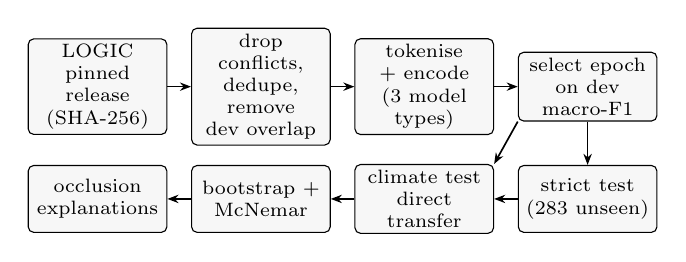
\begin{tikzpicture}[
  box/.style={draw, rounded corners=2pt, align=center, font=\scriptsize, minimum height=0.85cm, text width=1.62cm, inner sep=2pt, fill=gray!6},
  arr/.style={-{Stealth[length=4pt]}, semithick}]
\node[box] (raw) {LOGIC\\pinned release\\(SHA-256)};
\node[box, right=0.3cm of raw] (clean) {drop conflicts,\\dedupe, remove\\dev overlap};
\node[box, right=0.3cm of clean] (enc) {tokenise\\+ encode\\(3 model types)};
\node[box, right=0.3cm of enc] (sel) {select epoch\\on dev\\macro-F1};
\node[box, below=0.55cm of sel] (strict) {strict test\\(\nStrict{} unseen)};
\node[box, left=0.3cm of strict] (clim) {climate test\\direct transfer};
\node[box, left=0.3cm of clim] (stats) {bootstrap +\\McNemar};
\node[box, left=0.3cm of stats] (expl) {occlusion\\explanations};
\draw[arr] (raw) -- (clean);
\draw[arr] (clean) -- (enc);
\draw[arr] (enc) -- (sel);
\draw[arr] (sel) -- (strict);
\draw[arr] (sel.south west) -- (clim.north east);
\draw[arr] (strict) -- (clim);
\draw[arr] (clim) -- (stats);
\draw[arr] (stats) -- (expl);
\end{tikzpicture}
\caption{Experimental pipeline. Test labels enter only at the evaluation stage.}
\label{fig:pipeline}
\end{figure}

\subsection{Metrics}
Macro-F1 over the 13 classes is the headline metric because it weights rare classes equally with common ones. We also report accuracy, which equals micro-F1 for single-label prediction and is therefore the closest analogue to the micro-F1 reported by Jin et al.~\cite{jin2022logical}. The two papers' numbers remain not directly comparable, since our strict test removes seen sentences and our training set is cleaned.

\section{Models}
All models read the same cleaned text and output a softmax distribution over 13 classes (Fig.~\ref{fig:models}).

\textbf{TF-IDF + LR.} Unigram and bigram TF-IDF features (minimum document frequency 2, sublinear term frequency) feed a multinomial logistic regression ($C=10$). It is a non-neural reference point.

\textbf{CNN.} Following Kim~\cite{kim2014cnn}, 100-dimensional embeddings learned from scratch pass through 100 filters each of widths 3, 4 and 5 with ReLU, global max pooling, dropout 0.5 and a linear layer (444K parameters). The tokenizer keeps punctuation and stopwords, because words such as \emph{all}, \emph{therefore} and \emph{if} often mark the reasoning pattern.

\textbf{BiLSTM-Att.} The same embeddings feed a bidirectional LSTM~\cite{hochreiter1997lstm} with 128 units per direction. Additive attention~\cite{bahdanau2015attention} pools the hidden states into one vector before dropout and the output layer.

\textbf{DistilBERT.} The pretrained \texttt{distilbert-base-uncased} checkpoint~\cite{sanh2019distilbert} is fine-tuned end to end. It is a six-layer distilled version of BERT~\cite{devlin2019bert} with 66M parameters, using its own WordPiece tokenizer (maximum 128 tokens) and the standard classification head on the first token.

\textbf{Class weighting.} Each model is also trained with cross-entropy weighted by $w_c = N/(K n_c)$, where $n_c$ is the number of training examples of class $c$, $N$ the training size and $K=13$; for TF-IDF the equivalent ``balanced'' option is used.

\begin{figure}[t]
\centering
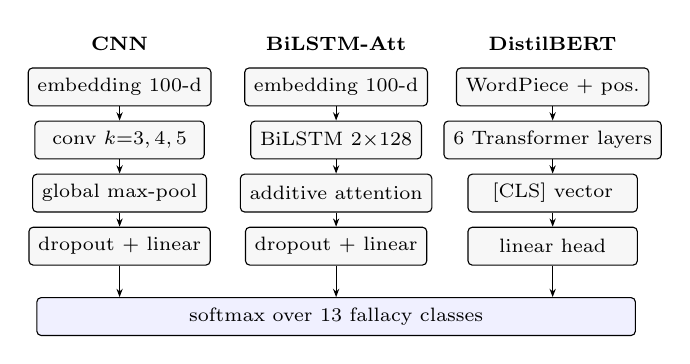
\begin{tikzpicture}[
  l/.style={draw, rounded corners=1.5pt, font=\scriptsize, minimum width=2.15cm, minimum height=0.48cm, fill=gray!6, align=center},
  arr/.style={-{Stealth[length=3pt]}},
  h/.style={font=\scriptsize\bfseries}]
\node[h] at (0,0.1) {CNN};
\node[l] (c1) at (0,-0.45) {embedding 100-d};
\node[l, below=0.18cm of c1] (c2) {conv $k{=}3,4,5$};
\node[l, below=0.18cm of c2] (c3) {global max-pool};
\node[l, below=0.18cm of c3] (c4) {dropout + linear};
\node[h] at (2.75,0.1) {BiLSTM-Att};
\node[l] (b1) at (2.75,-0.45) {embedding 100-d};
\node[l, below=0.18cm of b1] (b2) {BiLSTM $2{\times}128$};
\node[l, below=0.18cm of b2] (b3) {additive attention};
\node[l, below=0.18cm of b3] (b4) {dropout + linear};
\node[h] at (5.5,0.1) {DistilBERT};
\node[l] (t1) at (5.5,-0.45) {WordPiece + pos.};
\node[l, below=0.18cm of t1] (t2) {6 Transformer layers};
\node[l, below=0.18cm of t2] (t3) {[CLS] vector};
\node[l, below=0.18cm of t3] (t4) {linear head};
\foreach \a/\b in {c1/c2,c2/c3,c3/c4,b1/b2,b2/b3,b3/b4,t1/t2,t2/t3,t3/t4} \draw[arr] (\a) -- (\b);
\node[l, minimum width=7.6cm, below=0.4cm of b4, fill=blue!6] (soft) {softmax over 13 fallacy classes};
\foreach \x in {c4,b4,t4} \draw[arr] (\x) -- (\x |- soft.north);
\end{tikzpicture}
\caption{The three neural architectures compared in this study.}
\label{fig:models}
\end{figure}

\section{Experimental Setup}
CNN and BiLSTM are trained with Adam~\cite{kingma2015adam} (learning rate $10^{-3}$, batch 32) for at most 20 epochs with patience 4 on dev macro-F1, and inputs are truncated at 54 tokens, the 95th percentile of training length. DistilBERT is trained with AdamW~\cite{loshchilov2019adamw} (learning rate $5\times10^{-5}$, weight decay 0.01, batch 16, 10\% linear warm-up, gradient clipping at 1.0, mixed precision) for 8 epochs, keeping the epoch with the best dev macro-F1. The vocabulary for the non-pretrained models is built from training text only (minimum frequency 2). Every configuration is run with seeds 42, 43 and 44 on a single NVIDIA RTX 3050 laptop GPU with PyTorch 2.14. For significance we use seed-42 predictions on the strict test: a paired bootstrap with 2{,}000 resamples of the macro-F1 difference~\cite{efron1993bootstrap} and an exact McNemar test on discordant predictions~\cite{mcnemar1947,dietterich1998approximate}.

\section{Results}

\begin{table*}[t]
\centering
\caption{Main results (mean $\pm$ std over 3 seeds). Strict test excludes every test text seen in train or dev. Climate is direct transfer with no climate training. cw = class-weighted loss.}
\label{tab:main}
\setlength{\tabcolsep}{4pt}
\begin{tabular}{lrrcccc}
\toprule
Model & Params & Train (s) & Dev M-F1 & Strict Acc & Strict M-F1 & Climate M-F1 \\
\midrule
TF-IDF + LR & 101K & 2 & 0.489 $\pm$ 0.000 & 0.523 $\pm$ 0.000 & 0.473 $\pm$ 0.000 & 0.127 $\pm$ 0.000 \\
TF-IDF + LR (cw) & 101K & 1 & 0.498 $\pm$ 0.000 & 0.523 $\pm$ 0.000 & 0.475 $\pm$ 0.000 & 0.128 $\pm$ 0.000 \\
CNN & 437K & 13 & 0.444 $\pm$ 0.026 & 0.473 $\pm$ 0.016 & 0.423 $\pm$ 0.028 & 0.078 $\pm$ 0.012 \\
CNN (cw) & 437K & 8 & 0.449 $\pm$ 0.035 & 0.464 $\pm$ 0.007 & 0.426 $\pm$ 0.012 & 0.090 $\pm$ 0.034 \\
BiLSTM-Att & 584K & 10 & 0.391 $\pm$ 0.022 & 0.419 $\pm$ 0.014 & 0.358 $\pm$ 0.014 & 0.116 $\pm$ 0.007 \\
BiLSTM-Att (cw) & 584K & 9 & 0.357 $\pm$ 0.046 & 0.346 $\pm$ 0.086 & 0.333 $\pm$ 0.091 & 0.083 $\pm$ 0.028 \\
DistilBERT & 67.0M & 130 & 0.621 $\pm$ 0.010 & 0.585 $\pm$ 0.008 & 0.533 $\pm$ 0.008 & 0.133 $\pm$ 0.024 \\
DistilBERT (cw) & 67.0M & 123 & 0.632 $\pm$ 0.017 & 0.603 $\pm$ 0.005 & \textbf{0.554 $\pm$ 0.010} & 0.146 $\pm$ 0.013 \\
\bottomrule
\end{tabular}
\end{table*}


\subsection{Main comparison}
Table~\ref{tab:main} gives the full results. The two DistilBERT variants are the best models on every in-domain measure. The class-weighted variant has the highest dev macro-F1 (\devBertCw{}) and is therefore our selected model; on the strict test it reaches macro-F1 \fBertCw{}\,$\pm$\,\sdBertCw{} and accuracy \accBertCw{}, and the unweighted variant reaches \fBert{}\,$\pm$\,\sdBert{}. Selection uses the dev set only, so the choice does not rely on test data. The TF-IDF baseline is the best model without pretraining (\fTfidf{}), ahead of both neural models trained from scratch: the CNN reaches \fCnn{}\,$\pm$\,\sdCnn{} and the BiLSTM \fLstm{}\,$\pm$\,\sdLstm{}. A bag of n-grams therefore beats learned embeddings when only \nTrain{} training sentences are available, and the extra sequence modelling of the BiLSTM does not pay off at this scale. The non-pretrained models also vary more across seeds, which is expected given random embedding initialisation on a small corpus.

On the official test, which still contains the \nSeen{} previously seen sentences, every learned model scores higher than on the strict subset (DistilBERT-cw \offBertCw{}, CNN \offCnn{}). The two subsets differ in composition, so the gap is not a pure memorisation estimate, but it shows that reported LOGIC numbers depend on how overlap is handled.

Fig.~\ref{fig:comparison} places in-domain and transfer scores side by side. Training time grows from about a second for TF-IDF to roughly \timeBert{}\,s per DistilBERT run on a laptop GPU, which is still cheap enough for repeated seeds.

\begin{figure}[t]
\centering
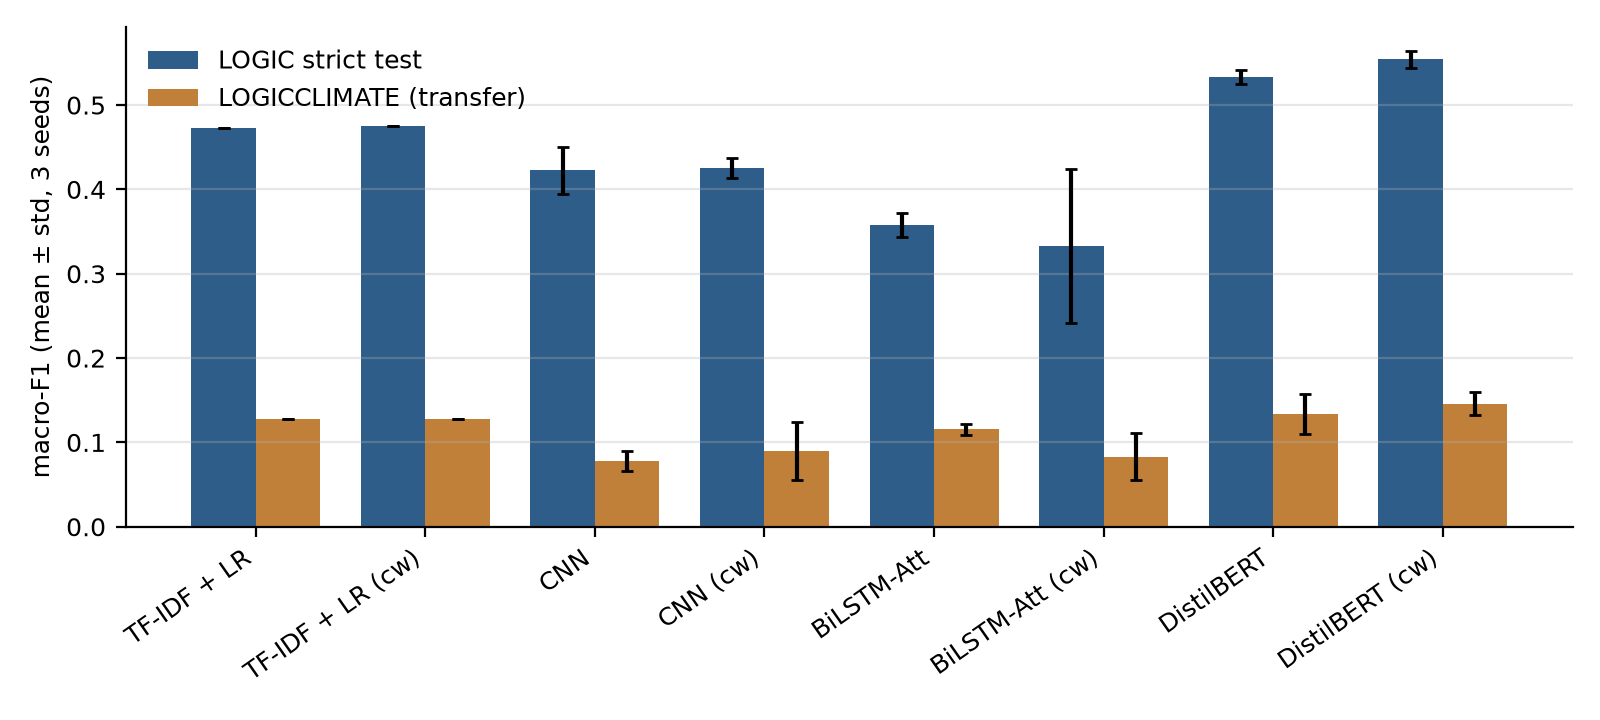
\includegraphics[width=\columnwidth]{../figures/final/model_comparison.png}
\caption{Strict-test and LOGICCLIMATE macro-F1 (mean $\pm$ std over \nSeeds{} seeds).}
\label{fig:comparison}
\end{figure}

\subsection{Is the difference real?}
Table~\ref{tab:sig} compares the selected model with every other configuration on the same strict-test rows. Against all TF-IDF, CNN and BiLSTM variants the paired bootstrap interval excludes zero and McNemar's test gives $p<0.01$, so the advantage of the pretrained encoder is not explained by test-set sampling. Against unweighted DistilBERT the difference is small and not significant under McNemar's test, so class weighting should be read as a minor refinement rather than a separate result.

\begin{table}[t]
\centering
\caption{Paired comparison of DistilBERT (cw) against each model on the strict test (seed 42): macro-F1 difference, 95\% paired-bootstrap interval (2{,}000 resamples) and exact McNemar $p$.}
\label{tab:sig}
\setlength{\tabcolsep}{4pt}
\begin{tabular}{lccc}
\toprule
Versus & $\Delta$M-F1 & 95\% CI & $p$ \\
\midrule
TF-IDF + LR & +0.087 & [+0.034, +0.146] & 0.002 \\
TF-IDF + LR (cw) & +0.085 & [+0.030, +0.141] & 0.004 \\
CNN & +0.143 & [+0.080, +0.205] & $<$0.001 \\
CNN (cw) & +0.124 & [+0.067, +0.182] & $<$0.001 \\
BiLSTM-Att & +0.201 & [+0.131, +0.270] & $<$0.001 \\
BiLSTM-Att (cw) & +0.163 & [+0.094, +0.227] & $<$0.001 \\
DistilBERT & +0.036 & [+0.002, +0.074] & 0.122 \\
\bottomrule
\end{tabular}
\end{table}


\subsection{Per-class behaviour and imbalance}
\begin{table}[t]
\centering
\caption{Per-class strict-test F1 (seed mean) for CNN and DistilBERT (cw), ordered by training frequency $n$.}
\label{tab:perclass}
\begin{tabular}{lrcc}
\toprule
Class & $n$ & CNN & DistilBERT (cw) \\
\midrule
faulty generalization & 314 & 0.52 & 0.64 \\
ad hominem & 219 & 0.56 & 0.74 \\
false causality & 167 & 0.43 & 0.65 \\
ad populum & 150 & 0.62 & 0.76 \\
circular reasoning & 131 & 0.58 & 0.55 \\
appeal to emotion & 127 & 0.37 & 0.50 \\
fallacy of logic & 119 & 0.32 & 0.39 \\
fallacy of relevance & 111 & 0.25 & 0.49 \\
intentional & 110 & 0.27 & 0.30 \\
false dilemma & 109 & 0.74 & 0.85 \\
fallacy of credibility & 107 & 0.18 & 0.47 \\
fallacy of extension & 100 & 0.57 & 0.60 \\
equivocation & 37 & 0.07 & 0.28 \\
\bottomrule
\end{tabular}
\end{table}

Table~\ref{tab:perclass} and Fig.~\ref{fig:perclass} break the scores down by class. Frequency is not the only factor. \emph{False dilemma}, a mid-frequency class with a distinctive surface form (``either \ldots\ or''), is the easiest class for the selected model, while \emph{equivocation}, the rarest class with 37 training sentences, remains the hardest for every model. The broad ``fallacy of'' categories (\emph{logic}, \emph{relevance}, \emph{credibility}) and \emph{intentional} are weak across the board. These labels are defined by what the argument does rather than by recognisable wording, and they overlap with more specific classes. The most frequent errors of the seed-42 DistilBERT model confirm this: \emph{faulty generalization} predicted as \emph{fallacy of logic}, and \emph{fallacy of relevance} predicted as \emph{fallacy of extension}.

Class weighting was expected to help rare classes. Its effect depends on the model (Fig.~\ref{fig:cw}): it gives DistilBERT a small gain spread over several classes, barely changes the CNN on average and hurts the BiLSTM, whose seed variance also grows. It never lifts \emph{equivocation} or \emph{intentional} above 0.30 F1. With fewer than 40 examples, reweighting the loss cannot supply the missing variety of phrasings.

\begin{figure*}[t]
\centering
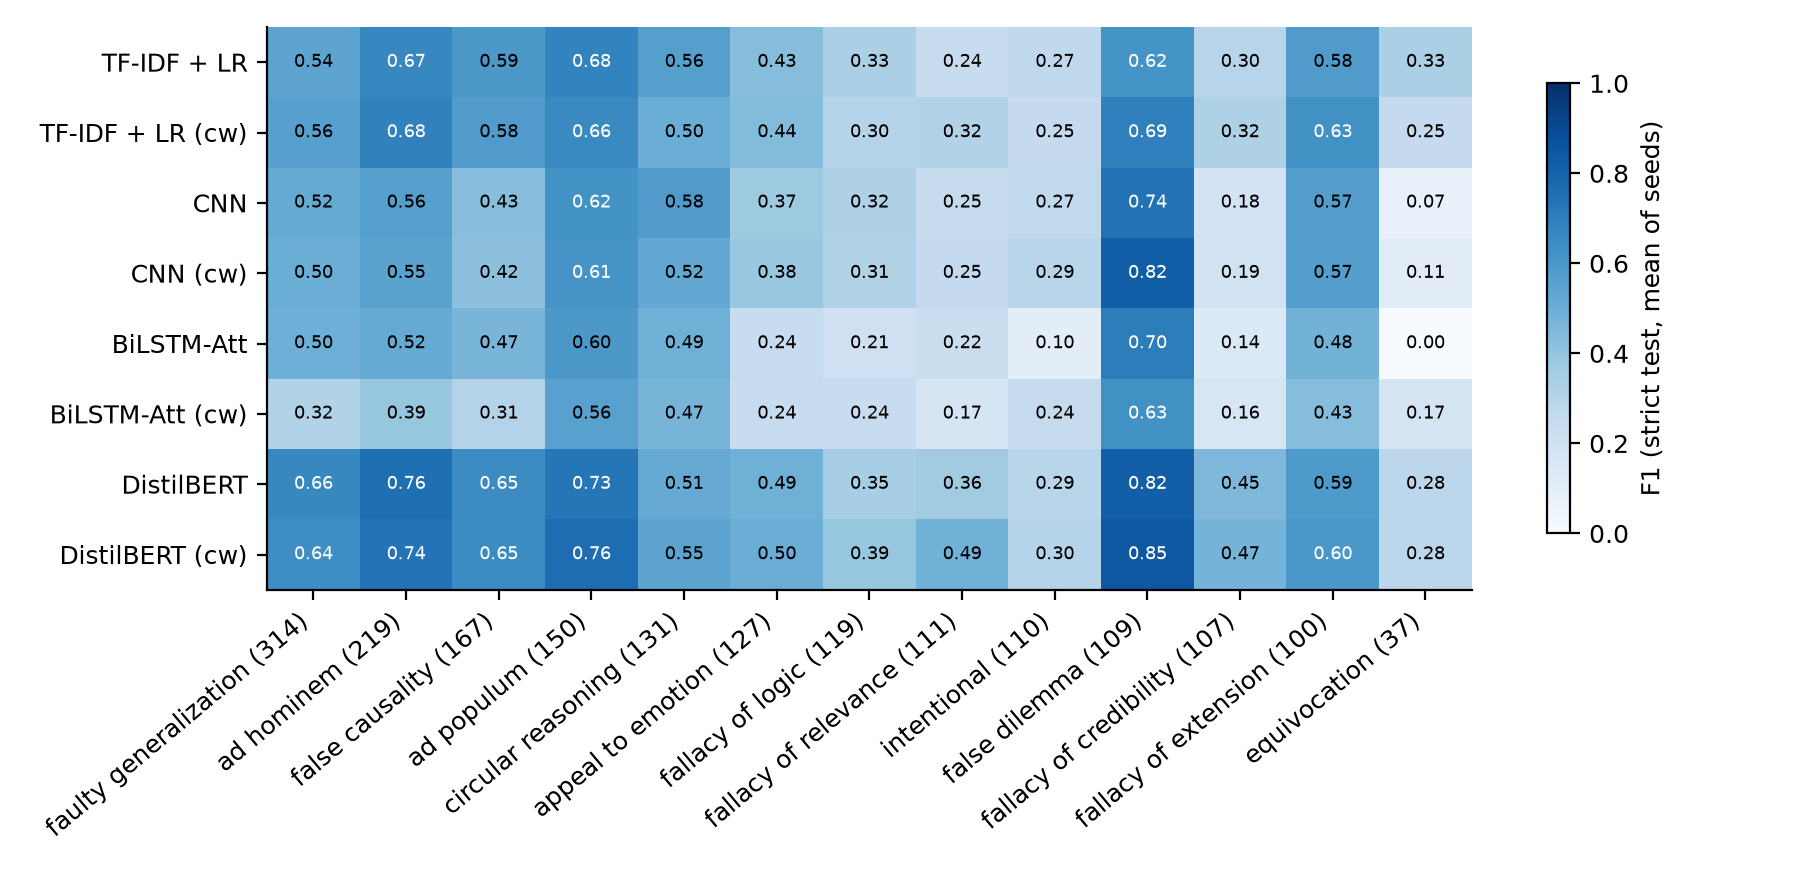
\includegraphics[width=0.85\textwidth]{../figures/final/per_class_f1.png}
\caption{Per-class strict-test F1 (seed mean). Columns are ordered by training frequency, shown in brackets.}
\label{fig:perclass}
\end{figure*}

\begin{figure}[t]
\centering
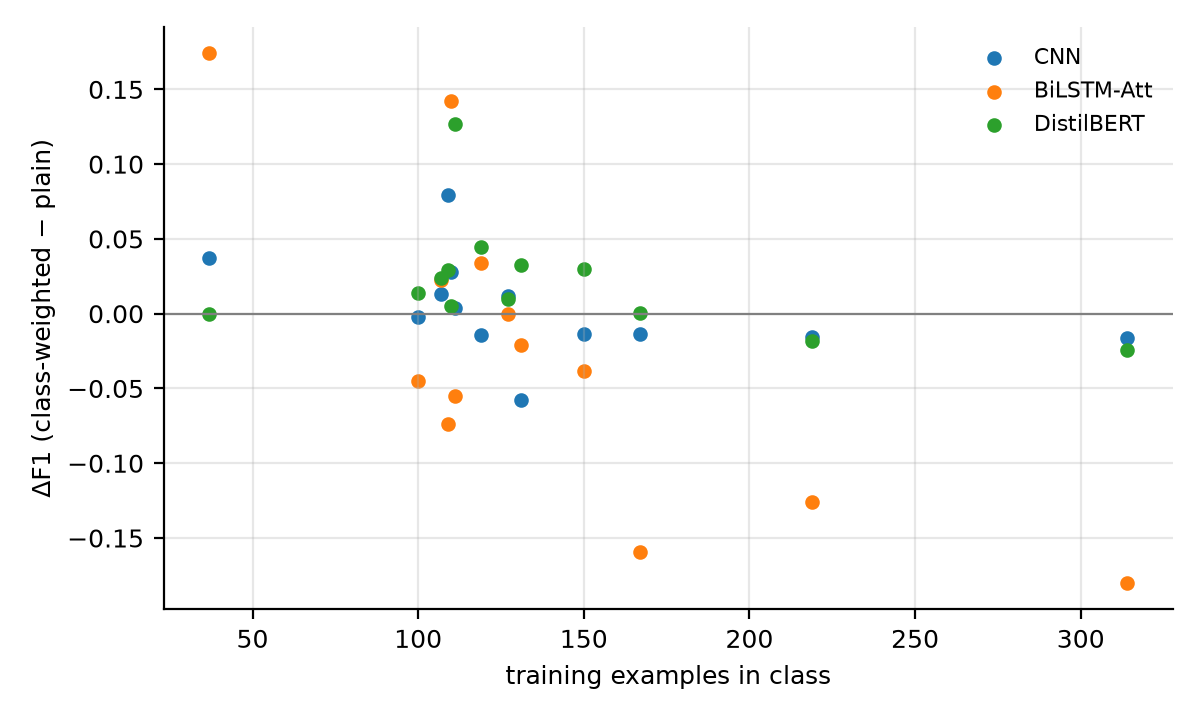
\includegraphics[width=0.92\columnwidth]{../figures/final/class_weighting_effect.png}
\caption{Change in per-class F1 from class weighting, plotted against class frequency.}
\label{fig:cw}
\end{figure}

\subsection{Transfer to climate news}
Applied without adaptation to LOGICCLIMATE, every model collapses (Table~\ref{tab:main}, last column). The best transfer macro-F1 is \climBertCw{} for class-weighted DistilBERT and \climTfidf{} for TF-IDF; the CNN falls to \climCnn{}. Climate sentences come from journalism rather than quizzes and follow a different label distribution in which \emph{intentional} is the most common class. Jin et al.\ reported a similar drop for their structure-aware model~\cite{jin2022logical}. In-domain gains therefore do not carry over to real discourse, and domain adaptation remains the main open problem for this line of work.

\subsection{Explanations}
For each prediction the interface removes one word at a time and records the drop in the predicted class's probability, a text version of occlusion analysis~\cite{zeiler2014visualizing}. We ran this probe over the correctly classified strict-test sentences of five classes with the seed-42 DistilBERT model and counted each sentence's two most influential words. For \emph{ad populum} the word \emph{everyone} was among them in 11 sentences; for \emph{false dilemma}, \emph{or} appeared 7 times and \emph{either} 3 times; for \emph{circular reasoning}, \emph{because} appeared 7 times. These are exactly the surface cues a human would point to. Such scores are useful for spotting shortcut cues, but they measure sensitivity rather than reasoning, and we do not use them as evidence that a model understands the argument.

\begin{figure}[t]
\centering
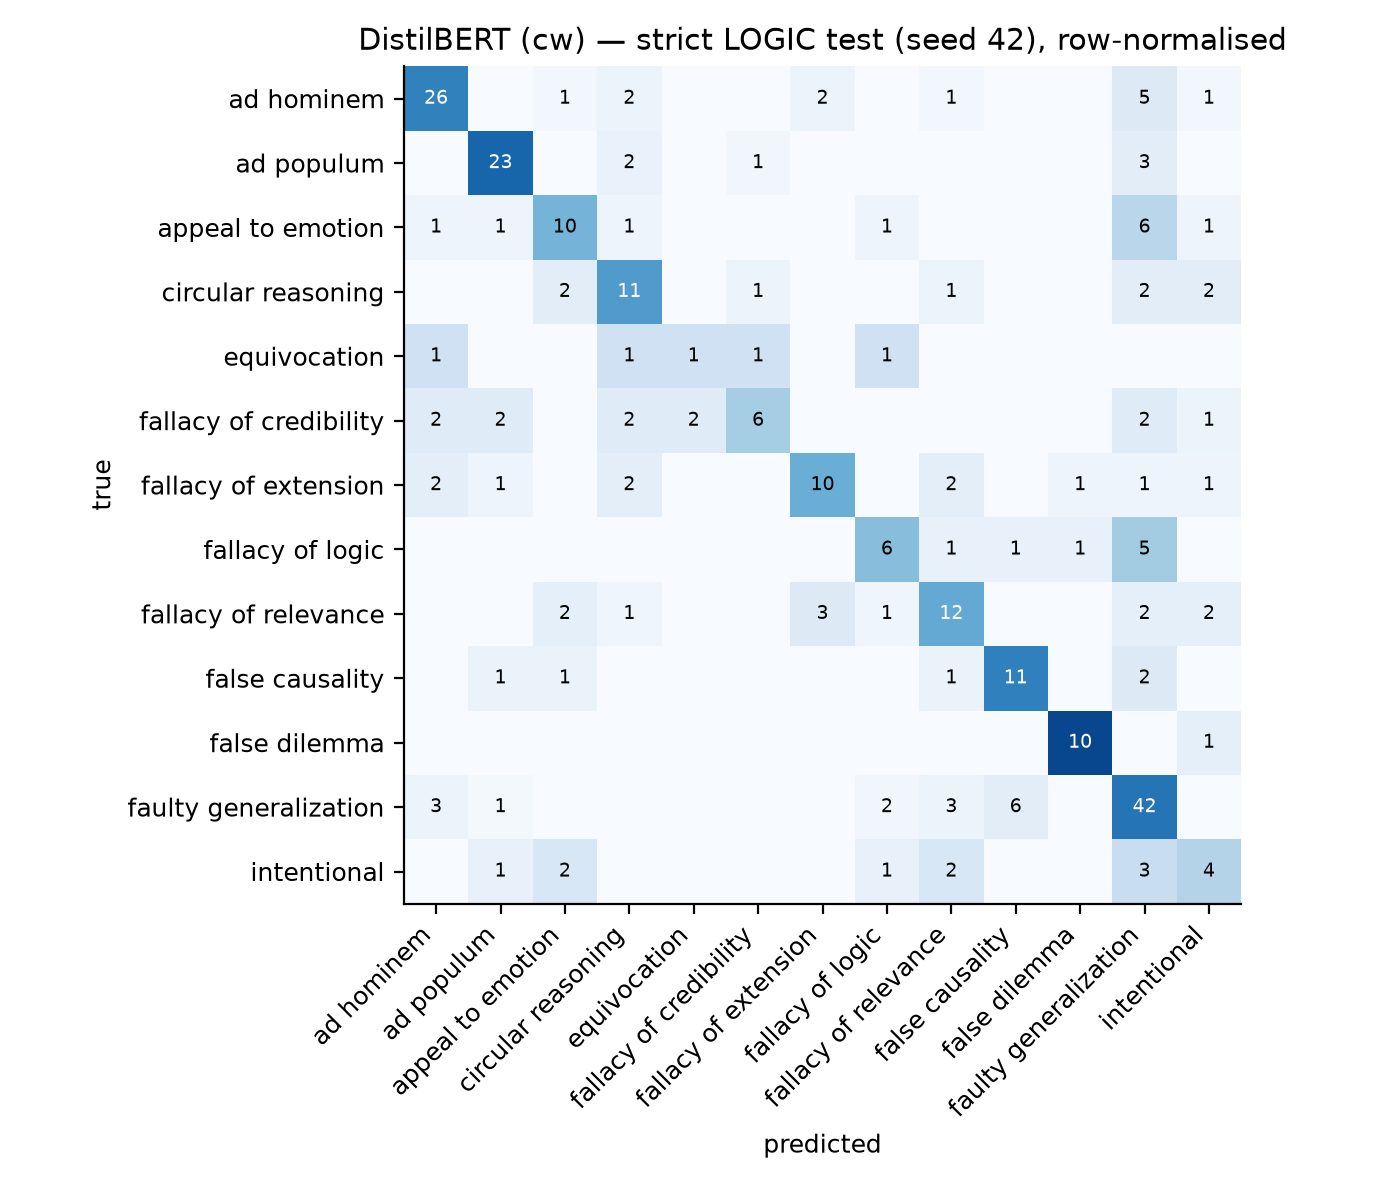
\includegraphics[width=0.95\columnwidth]{../figures/final/confusion_matrix_selected.png}
\caption{Row-normalised confusion matrix of the selected model (DistilBERT, class-weighted) on the strict test (seed 42); cells show counts.}
\label{fig:cm}
\end{figure}


\section{Limitations and Responsible Use}
LOGIC is small and drawn mostly from educational material, so even strict-test scores describe performance on textbook-style examples. The label set has no ``no fallacy'' class: any input, including a sound argument, receives one of 13 fallacy labels, which rules out unsupervised deployment as a detector. The released rows are single-label although real arguments can commit several fallacies at once~\cite{helwe2024mafalda}. We tested one pretrained model size and three seeds; larger encoders, more seeds or a tuning budget could change the margins. Occlusion scores show what a model is sensitive to, not why an argument is fallacious. For these reasons the accompanying interface presents predictions as hypotheses with probabilities and explanations, and states that it does not judge truth.

\section{Conclusion}
We compared four families of text classifiers on LOGIC under a protocol that removes conflicting labels, eliminates train/dev overlap and scores models on \nStrict{} test sentences none of them had seen. Fine-tuned DistilBERT was the strongest model, with strict macro-F1 \fBertCw{} for the selected class-weighted variant, and its margin over TF-IDF, CNN and BiLSTM held under paired significance tests. A TF-IDF linear model beat both neural networks trained from scratch, so on a corpus of this size pretraining, not architecture, is what separates the models. Class weighting brought at most a small gain and did not fix the weakest classes, which are the rare and loosely defined ones. No model transferred to climate-news fallacies. Future work should evaluate larger encoders and more seeds, add a non-fallacious class so that the task covers detection as well as classification, and test domain adaptation on naturally occurring corpora such as CoCoLoFa and MAFALDA.


\section*{Code and Data Availability}
Code, saved per-seed predictions, figures and the web interface are available in the project repository (\url{https://github.com/lakshitsachdeva/fallacydetection}). LOGIC and LOGICCLIMATE are available from the original authors at \url{https://github.com/causalNLP/logical-fallacy}.

\bibliographystyle{IEEEtran}
\bibliography{refs}

\end{document}
